
%
\documentclass[%
 reprint,
 amsmath,amssymb,
 aps,
]{revtex4-1}

\usepackage{graphicx}% Include figure files
\usepackage{dcolumn}% Align table columns on decimal point
\usepackage{bm}% bold math


\begin{document}



\title{Sistema de Gestion para el concurso de Proyectos de la EPIS}
\author{Jose Pastor Mendoza}
\author{Arlyn Cotrado Coaquira}
\author{Andrés De La Barra Vasquez}
\affiliation{%
 Universidad Privada de Tacna \textbackslash Facultad de Ingenieria \textbackslash Escuela Profesional de Ingenieria de Sistemas
}%

\begin{abstract}
\begin{center}
\textbf{Resumen}
\end{center}
Balanced Scorecard y Business model canvas son técnicas de análisis empresarial . Ambas técnicas son útiles para mejorar el desempeño organizacional. Pero sus aplicaciones difieren. Ambos se pueden usar junto con los indicadores clave de rendimiento para monitorear y mejorar el rendimiento de la organización. Vamos a entender tanto la técnica en detalle.


\begin{center}
\textbf{Abstract}
\end{center}
Balanced Scorecard and Business model canvas are business analysis techniques. Both techniques are useful to improve organizational performance. But their applications differ. Both can be used together with the key performance indicators to monitor and improve the performance of the organization. We will understand both the technique and the detail.

\end{abstract}



\maketitle

%\tableofcontents

\section {Introducción}

El BSC retiene las medidas financieras tradicionales que se combinan con la metodología del EVA y se complementan con indicadores de desempeño futuro.\\
Ésta es una metodología útil para la implementación estratégica que “traduce” la misión, la visión y la estrategia de las diferentes unidades de negocio de la\\
empresa en objetivos e indicadores tangibles, los cuales son agrupados en forma de causa y efecto, en cuatro perspectivas que permiten visualizar el desempeño\\
organizacional: perspectiva financiera, clientes, procesos internos y crecimiento y aprendizaje.\\

El BSC sugiere que las medidas financieras y no financieras deben ser parte del sistema de información para los empleados de todos los\\
niveles de la organización. Aquellos de niveles inferiores podrán entender el efecto financiero de sus decisiones, mientras que los de niveles superiores podrán\\
entender los impulsores del efecto financiero a largo plazo.\\


%-----------------------------------------------------------------
\section {Objetivos}
\begin{itemize}
\item Integrar todas las actividades involucradas en el proceso del concurso de proyectos de la EPIS. \\
\item Facilitar a todos los usuarios el proceso que les corresponda realizar segun su rol. \\
\item Investigar el uso de tecnologias web para la realizacion del proyecto.  \\
\item Crear un producto completo para mejorar tiempos y organizar procesos .\\
\end{itemize}

\section {Problematica}
Lorem ipsum dolor sit amet, consectetur adipiscing elit. Quisque porta, sem eget lobortis bibendum, orci risus interdum sapien, quis pellentesque leo libero ac erat. Donec quis odio lorem. In hendrerit eget lectus sed ornare. Pellentesque rutrum velit eget orci semper molestie. Sed tincidunt sodales posuere. Sed sapien elit, tempus eu cursus at, ornare eget felis. Donec in dignissim odio.

Suspendisse velit massa, venenatis nec dolor a, consectetur pharetra nisl. Morbi dignissim massa sed orci elementum, at molestie lectus elementum. Fusce sit amet laoreet lectus. Phasellus ut aliquam mauris, eu faucibus magna. In eget vulputate ligula, quis euismod augue. Sed id hendrerit ante. Suspendisse efficitur leo diam, quis placerat arcu finibus vel. Integer viverra sodales neque, ac viverra velit. Nunc efficitur fringilla nulla. Nulla vel imperdiet magna. Suspendisse imperdiet neque velit, vitae rhoncus ligula mattis non.

\section {Desarrollo de la solucion}

Lorem ipsum dolor sit amet, consectetur adipiscing elit. Quisque porta, sem eget lobortis bibendum, orci risus interdum sapien, quis pellentesque leo libero ac erat. Donec quis odio lorem. In hendrerit eget lectus sed ornare. Pellentesque rutrum velit eget orci semper molestie. Sed tincidunt sodales posuere. Sed sapien elit, tempus eu cursus at, ornare eget felis. Donec in dignissim odio.

Suspendisse velit massa, venenatis nec dolor a, consectetur pharetra nisl. Morbi dignissim massa sed orci elementum, at molestie lectus elementum. Fusce sit amet laoreet lectus. Phasellus ut aliquam mauris, eu faucibus magna. In eget vulputate ligula, quis euismod augue. Sed id hendrerit ante. Suspendisse efficitur leo diam, quis placerat arcu finibus vel. Integer viverra sodales neque, ac viverra velit. Nunc efficitur fringilla nulla. Nulla vel imperdiet magna. Suspendisse imperdiet neque velit, vitae rhoncus ligula mattis non.
\begin{center}
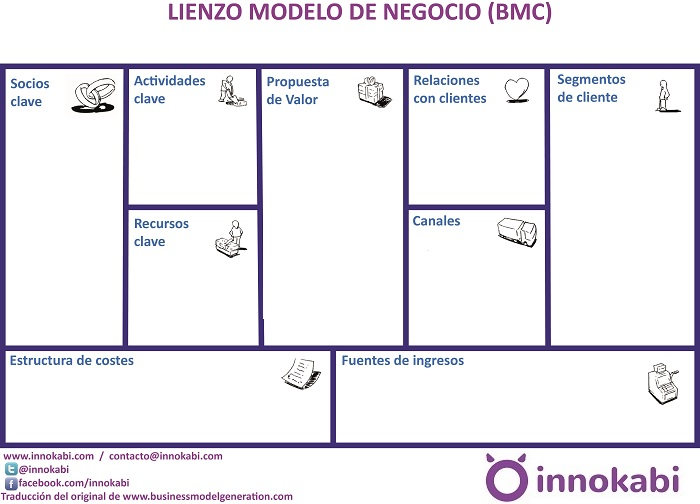
\includegraphics[width=10cm]{./Imagenes/imagen4}
\end{center}

%-----------------------------------------------------------------
\section{Conclusiones}

\begin{itemize}
\item El Balanced Scorecard nos ayuda a establecer y enfocar las estratégias de la empresa hacia el futuro, todo con el fin de poder convertir en realidad la visión empresarial, esto se logra a través de la suma de los objetivos de cada una de las cuatro perspectivas que nos propone mejorar el BSC.

\item Balanced Scorecard y Business model canvas son técnicas de análisis empresarial. Ambas técnicas son útiles para mejorar el desempeño organizacional. . Ambos se pueden usar junto con los indicadores clave de rendimiento para monitorear y mejorar el rendimiento de la organización. 

\end{itemize}

% Bibliografia.
%-----------------------------------------------------------------

%\bibliographystyle{plain}
%\bibliography{Bibliografia}

\end{document}

